%%%%%%%%%%%%%%%%%%%%%%%%%%%%%%%%%%%%%%%%%%%%%%%%%%%%%%%%%%%%%%%%%%
%  = PREAMBLE =
% The preamble of a LaTeX document is the set of commands that 
%    precede the \begin{document} line.  It sets up the style of 
%    the document.
%%%%%%%%%%%%%%%%%%%%%%%%%%%%%%%%%%%%%%%%%%%%%%%%%%%%%%%%%%%%%%%%%%

\documentclass[aps,twocolumn, secnumarabic,balancelastpage,amsmath,amssymb,nofootinbib,floatfix]{revtex4-1}

\usepackage{graphicx}      % tools for importing graphics
\usepackage{tikz}
\usepackage{parskip}
\usepackage[colorlinks=true]{hyperref}  % this package should be added after 
                                        % all others.
                                        % usage: \url{http://web.mit.edu/8.13}

\setlength{\parskip}{5pt}
\usetikzlibrary{decorations.pathmorphing}

%%%%%%%%%%%%%%%%%%%%%%%%%%%%%%%%%%%%%%%%%%%%%%%%%%%%%%%%%%%%%%%%%%%
% And now, begin the document...
%%%%%%%%%%%%%%%%%%%%%%%%%%%%%%%%%%%%%%%%%%%%%%%%%%%%%%%%%%%%%%%%%%%

\begin{document}

\title{Compton Scattering Experiment Summary}
% \author{Vinh Tran}
% \email{vinhtran@mit.edu}
\author{Yongao Hu}
\email{yongao@mit.edu}
\date{\today}
\affiliation{MIT Department of Physics}


\begin{abstract}
This report presents the results of the Compton scattering experiment conducted in MIT Junior Lab during Spring 2025. The objective of the experiment was to measure the particle nature of light during scattering. The experiment was successful in demonstrating the particle nature of light. 
\end{abstract}

\maketitle

\section{Introduction}
Compton scattering, discovered by Arthur Compton in 1923, is the inelastic scattering of a photon by a charged particle, usually an electron. The experiment is a direct demonstration of the particle nature of light. 

In this experiment, we will measure the energy of the scattered photons and the recoiled electrons as a function of the scattering angle. The energy of the scattered photons will be measured using scintillation detectors. We will also measure the total cross section of the scattering process through measurements of attenuation of the photon beam as a function of the thickness of the attenuation material.

The paper will begin by discussing the theory of Compton scattering. We will then describe the experimental setup and the data analysis. Finally, we will present the results of the experiment and discuss the implications of the results. 

\section{Theory: Relativistic Scattering of Photons}
\subsection{Relativistic Kinematics of Scattering}
The Compton scattering can be explained if we treat the photon as a particle with energy $E = hf$ and momentum $p = hf/c$. 

In Einstein's special relativity, the energy and momentum of the photon are related by the equation $E^2 = p^2c^2 + m^2c^4$, where $m$ is the rest mass of the photon. 

When a photon scatters off an electron at rest, the photon transfers some of its energy and momentum to the electron. The energy and momentum of the scattered photon can be calculated using the conservation of energy and momentum from special relativity. 

We can write the equations for conservation of energy and momentum in two dimensions as: 
\begin{eqnarray}
E_i + m_e c^2 &=& E_f + E_e \\
\vec{p_i} &=& \vec{p_f} + \vec{p_e}
\end{eqnarray}
where $E_i$ and $\vec{p_i}$ are the energy and momentum of the incident photon, $E_f$ and $\vec{p_f}$ are the energy and momentum of the scattered photon, and $E_e$ and $\vec{p_e}$ are the energy and momentum of the recoiled electron.

If we use the rest frame of the initial electron and align the incident photon along the $x$-axis, as shown in Fig. \ref{fig:scattering}, we can write the momenta as
\begin{eqnarray}
\vec{p_i} &=& (E_i/c, 0) \\
\vec{p_f} &=& (E_f/c\cos\theta, E_f/c \sin\theta) \\
\vec{p_e} &=& (E_e/c\cos\phi, -E_e/c \sin\phi)
\end{eqnarray}
where $\theta$ is the scattering angle of the photon and $\phi$ is the scattering angle of the electron.

We then can solve the conservation equations to find the energy of the scattered photon:
\begin{equation}
E_f = \frac{E_i}{1 + \frac{E_i}{m_e c^2}(1 - \cos\theta)}
\end{equation}
where $\theta$ is the scattering angle.
\begin{figure}[h]
    \centering
    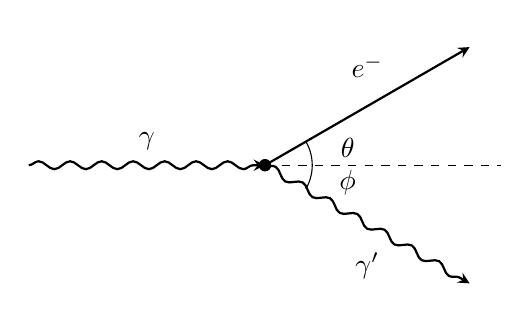
\begin{tikzpicture}[scale=1.5,>=stealth]
      % Draw the incident photon arrow (from left to the vertex)
      \draw[decorate, decoration={snake, amplitude=0.5mm, segment length=4mm}, thick, ->] (-2,0) -- (0,0) node[midway, above, inner sep=5] {$\gamma$};

      \draw[-, dashed] (0,0) -- (2,0);
      
      % Mark the scattering vertex
      \fill (0,0) circle (1.5pt);
      
      % Draw the scattered photon arrow (at theta=30°)
      \draw[decorate, decoration={snake, amplitude=0.5mm, segment length=4mm}, thick, ->] (0,0) -- (1.732,-1) node[midway, below,inner sep=10] {$\gamma'$};
      
      % Draw the recoil electron arrow (at phi=30° below horizontal)
      \draw[->, thick] (0,0) -- (1.732,1) node[midway, above,inner sep=10] {$e^-$};
      
      % Mark the scattering angle theta (arc from horizontal to photon arrow)
      \draw (0.4,0) arc (0:-30:0.4);
      \node at (0.7,0.15) {$\theta$};
      
      % Mark the recoil angle phi (arc from horizontal to electron arrow)
      \draw (0.4,0) arc (0:30:0.4);
      \node at (0.7,-0.15) {$\phi$};
    \end{tikzpicture}
    \caption{Compton scattering diagram showing the incident photon ($\gamma$), the scattered photon ($\gamma'$) deflected by an angle $\theta$, and the recoil electron ($e^-$) at an angle $\phi$.}
    \label{fig:scattering}
    \end{figure}

\subsection{Total Cross Section}
The total cross section of the Compton scattering process is the probability of the scattering process occurring. Classically, the total cross section of the Compton scattering process is given by the Thomson scattering formula:
\begin{equation}
\sigma(\theta) = \frac{8\pi}{3} r_0^2 \left( \frac{1 + \cos^2\theta}{2} \right)
\end{equation}
where $r_0$ is the classical electron radius.

Thomson scattering formula is derived from the classical electromagnetic theory and is valid for low-energy photons. However, when the energy of the photon is comparable to the rest mass of the electron, the relativistic effects become important.

If we include the relativistic effects, the total cross section of the Compton scattering process is given by the Klein-Nishina formula:
\begin{equation}
\sigma(\theta) = \frac{r_0^2}{2} \left( \frac{1 + \cos^2\theta}{1 + \gamma(1 - \cos\theta)} \right)
\end{equation}
where $r_0$ is the classical electron Bohr radius 
\begin{equation}
r_0 = \frac{e^2}{4\pi\epsilon_0 m_e c^2}
\end{equation}

and $\gamma = E_i/m_e c^2$ is the Lorentz factor of the incident photon.

\section{Experimental Design}
\subsection{Apparatus}
The source of the photons is a $^{137}$Cs radioactive source. The source emits photons with energy $E_i = 661$ keV. The experiment uses two scintillation detectors to measure the energy of the scattered photons. One scintillator is used as the target to scatter the photons, and the other scintillator is used to detect the scattered photons. We will call the scintillator that serves as a target and measure the energy of the recoiled electrons the ``recoil detector'' and the scintillator that measures the energy of the scattered photons the ``scatter detector''.

The scatter detector is placed at an angle $\theta$ with respect to the incident photon beam. The energy of the scattered photon is measured by the energy deposited in the scintillation detectors. 

In order to measure the total cross section of the Compton scattering process, we will use an absorber to attenuate the photon beam. The attenuation of the photon beam will be measured as a function of the thickness of the absorber.

\subsection{Circuit Design}
In order to make sure that we are not measuring the energy of the photons from the source, we will use a coincidence circuit to measure the energy of the scattered photons. The coincidence circuit will only output a signal when both detectors detect a photon within a short time window. 

The circuit diagram is shown in Fig. \ref{fig:circuit}. We feed the output from the scintillators into pre-amplifiers and amplifiers. The outputs of the amplifiers are connected to multichannel analyzers (MCA) to measure the energy of the scattered photons and recoiled electrons. The outputs of the amplifiers are also fed into a coincidence circuit: we first use inverters and discriminators to covert the pulses above a certain threshold from the amplifiers into square waves to reduce noise. The discriminated square waves are then fed into a coincidence circuit. The output of the coincidence circuit is connected to a delay generator to ensure that MCA has enough time to record the energy of the scattered photons and recoiled electrons. The output of the delay generator is connected to the gates of MCA to ensure that we are only measuring the energy from Compton scattering events and not from the source or stray radiation.

\subsection{Calibration}
As we do not know exactly the gains set by the circuit and hence what each bin of MCA correspond to in terms of energy, we need to calibrate the MCA. We use a $^{22}$Na source and a $^{133}$Ba source to calibrate the MCA. The $^{22}$Na source emits gamma rays with energies of 511 keV. The $^{133}$Ba source emits gamma rays with energies of 356 keV and 384 keV. We then fit a linear function between the channel number of the MCA and the energy of the gamma rays to calibrate the MCA.

\subsection{Angular Dependence of Scattering}
We measure the energy of the scattered photons as a function of the scattering angle $\theta$. We place the scatter detector at different angles with respect to the incident photon beam and measure the energy of the scattered photons. We then use the energy of the scattered photons to calculate the scattering angle $\theta$.

\subsection{Total Cross Section}
We measure the attenuation of the photon beam as a function of the thickness of the absorber. In particular, we are using polyvinyltoluene (PVT) as the absorber. Electrons in PVT are bounded at a much lower energy than the energy of the incident photons, hence can be considered as free electrons.

We place the absorber of different thickness in the path of the photon beam and measure the attenuation of the photon beam using the scatter detector. We then use the attenuation of the photon beam and fit an exponential decaying function to the data to calculate the total cross section of the Compton scattering process. 


\section{Data Analysis}
\subsection{Peak Fitting}
In order to find the peak of energy of the detected particles, we first use a Kernel Density Estimator (KDE) to smooth the data: we use a Gaussian kernel with a bandwidth of 10 keV. KDE fits a Gaussian function to each data point and then sums up the Gaussian functions to create a smooth curve. We use KDE to preliminarily find the peak of the energy of the detected particles. 

We then use a peak-finding algorithm to find the peak and valley of the energy of the detected particles. Afterwards, we fit a Gaussian function to the original data between the two adjacent valleys to find the peak. The area under the Gaussian function is proportional to the number of detected particles that we considered as ``detected'' by the detector. We will take the width of the Gaussian function as the uncertainty of the energy of the detected particles.

\subsection{Calibration}
After identifying the peak of the energy from the calibration sources, we fit a linear function between the channel number of the MCA and the energy of the gamma rays. Note that we calibrate the detectors separately as they may have different gains. We also calibrate them at the beginning of different sessions to account for the drift of the gains.

\subsection{Angular Dependence of Scattering}
After finding the peak of energy of the scattered photons at different angles, we can overlay them with theorectical predictions to verify the Compton scattering formula. We can also overlay the rate of the scattered photons with the Klein-Nishina formula to verify the total cross section of the Compton scattering process. 

\subsection{Total Cross Section}
We fit an exponential decaying function to the data of the attenuation of the photon beam as a function of the thickness of the absorber. We then extrapolate the fitted function to calculate the total cross section of the Compton scattering process. 

\section{Results}
\subsection{Angular Dependence of Scattering}
\subsubsection{Error Analysis of Angular Dependence}
At $\theta = 0$, theory predicts that the energy of the scattered photon is the same as the incident photon. However, due to alignment errors, our measurement of the energy of the scattered photon at $\theta = 0$ is not exactly the same as the incident photon. The alignment is a major source of systematic error in the experiment.

The statistical error of the data comes from the standard deviation from the peak-fitting algorithm. 

\subsection{Total Cross Section}
\subsubsection{Error Analysis of Total Cross Section}
With the measurement of the absorber, we introduce a systematic error from the uncertainty in the dimension of the absorber. The thickness of the absorber is measured using a ruler, which has an uncertainty of 1 mm. 

The statistical error of the data again comes from the standard deviation from the peak-fitting algorithm.



 

\section{Conclusion}
The Compton scattering experiment successfully demonstrated the particle nature of light. The experiment measured the energy of the scattered photons and recoiled electrons as a function of the scattering angle. The experiment also measured the total cross section of the Compton scattering process. The results of the experiment are consistent with the theoretical predictions of the Compton scattering process.

\begin{acknowledgments} The author gratefully acknowledges their lab partner V. Tran for their invaluable assistance. The author also thanks the 8.13 teaching team for their guidance in the lab. This work was supported by the MIT Department of Physics. 
\end{acknowledgments}

% \bibliographystyle{abbrv}
% \bibliography{ref}
\end{document}

